% This text is proprietary.
% It's a part of presentation made by myself.
% It may not used commercial.
% The noncommercial use such as private and study is free
% Sep. 2005 
% Author: Sascha Frank 
% University Freiburg 
% www.informatik.uni-freiburg.de/~frank/


\documentclass{beamer}


\newcommand{\xk}{{{x}^{(k)}}}
\newcommand{\dk}{{\Delta_k}}
\newcommand{\mk}{{m_f}}
\newcommand{\fk}{{f_k}}
\newcommand{\fgk}{{g^{(k)}_f}}
\newcommand{\fhk}{{H^{(k)}_f}}
\newcommand{\ck}{{c^{(k)}_{i}(\xk)}}
\newcommand{\cgk}{{g^{(k)}_{c_i}}}
\newcommand{\mck}{{m_{c_i}}}
\newcommand{\bk}{{B_{\infty}(\xk, \dk)}}



\usepackage{color}


\begin{document}


\title{Master's Presentation}   
\author{Trever} 
\date{\today} 

\frame{\titlepage} 

\section{Introduction}

\begin{frame}{Introduction}
    \begin{itemize}
        \item We develop an algorithm to find local optima of convex constrained problems
        \item This algorithm is useful for problems where function values are not provided for infeasible points
        \item The focus is on narrow feasible regions
    \end{itemize}
\end{frame}

\section{Derivative Free Background}

\begin{frame}{Derivative Free Problem Formulation}
\begin{center}
\label{Problem}
\begin{align*}
\min_x & \quad f(x) \\
  c_i(x) \le 0   & \quad \forall \; 1 \le i \le m \\
\end{align*}
\end{center}
    \begin{itemize}
        \item All functions are black-box functions, meaning that we have no information about their derivatives
        \item For example, optimization problems where the objective or some of the constraints depend on an expensive simulation
        \item Function values may not be available outside of the feasible region, we call this \emph{partially-quantifiable}
%        \item $S(x)$ is a black-box function, meaning that we have no information about its derivatives
%        \item We assume that $f$ and $c$ are apriori functions
%         \item We assume the level sets of $f$ are bounded
%         \item We assume $f$, $c$ are continuously twice differentiable
%         \item The goal of my research is to develop algorithms for this problem
    \end{itemize}
\end{frame}


\begin{frame}{Strategy}
    \begin{itemize}
        \item Extend our current algorithm for solving linear partially-quantifiable constraints to convex constraints
        \item Account for uncertainty in constraint boundaries
        \item Ensure that no infeasible points must be evaluated
    \end{itemize}
\end{frame}


\frame{\frametitle{Table of Contents}\tableofcontents} 



\begin{frame}{Model Based Trust Region Methods}
    \begin{itemize}
        \setlength\itemsep{2em}
    	\item Approximate $f$ and $c$ in terms of model functions
    	\item We approximate using a second order model, meaning that we approximate:
    	\begin{itemize}
            \item $\fhk \approx \nabla ^2 f(\xk)$
            \item $\fgk \approx \nabla f(\xk)$
            \item $\mk(x) = \fk + \left(x - \xk \right)^T\fgk + \left(x - \xk \right)^T\fhk\left(x - \xk \right) \approx f(x)$
            \item $\cgk \approx c_i(\xk)$
            \item $\mck(x) = \ck + \left(x - \xk\right)^T\cgk \approx c_i(\xk)$
    	\end{itemize}
	    \item Choose next iterate by minimizing a model problem over a trust region
	\end{itemize}
\end{frame}



% 12
\begin{frame}{Trust Region Subproblem}
    \begin{itemize}
        \item In each iteration, we attempt to solve the trust region subproblem to compute a step direction $s$

        \begin{displaymath}
\begin{array}{lrcc}
min_s & \mk(s)   &     &            \\
s.t.  &  \mck(x) & \le & 0   \quad \forall \; 1 \le i \le m       \\
      &  s & \in & \bk.  \\
\end{array}
        \end{displaymath}
    \end{itemize}
\end{frame}





%\begin{frame}{Trust Region Management}
%    \setlength\itemsep{2em}
%    \begin{itemize}
%		\item $\rho_k = \frac{f(x^{(k)}) - f(x^{(k)}+s^{(k)})}{m_k(x^{(k)}) - m_k(x^{(k)}+s^{(k)})}$
%        \item This is the actual decrease over the predicted decrease
%        \begin{itemize}
%            \item measures accuracy of model functions
%            \item ensures reduction in the objective
%        \end{itemize}
%        \item Helps determine new trust region radius
%		\begin{itemize}
%		    \item If $\rho_k$ is small, $x^{(k+1)}=x^{(k)}$ (reject) and decrease radius
%		    \item If $\rho_k$ is intermediate, $x^{(k+1)}=x^{(k)}+s^{(k)}$ (accept) and decrease radius
%		    \item If $\rho_k$ is large, $x^{(k+1)}=x^{(k)}+s^{(k)}$ (accept) and increase radius
%		\end{itemize}
%        \item There are several potential approaches for incorporating constraints
%    \end{itemize}
%\end{frame}


\begin{frame}{Geometry}
    \begin{itemize}
        \item<1, 2, 3> Geometry refers to the shape of the set of sample points
        \item<1, 2, 3> When the points are not well poised, the constructed model can be innacurate \\
        \only<2>{
            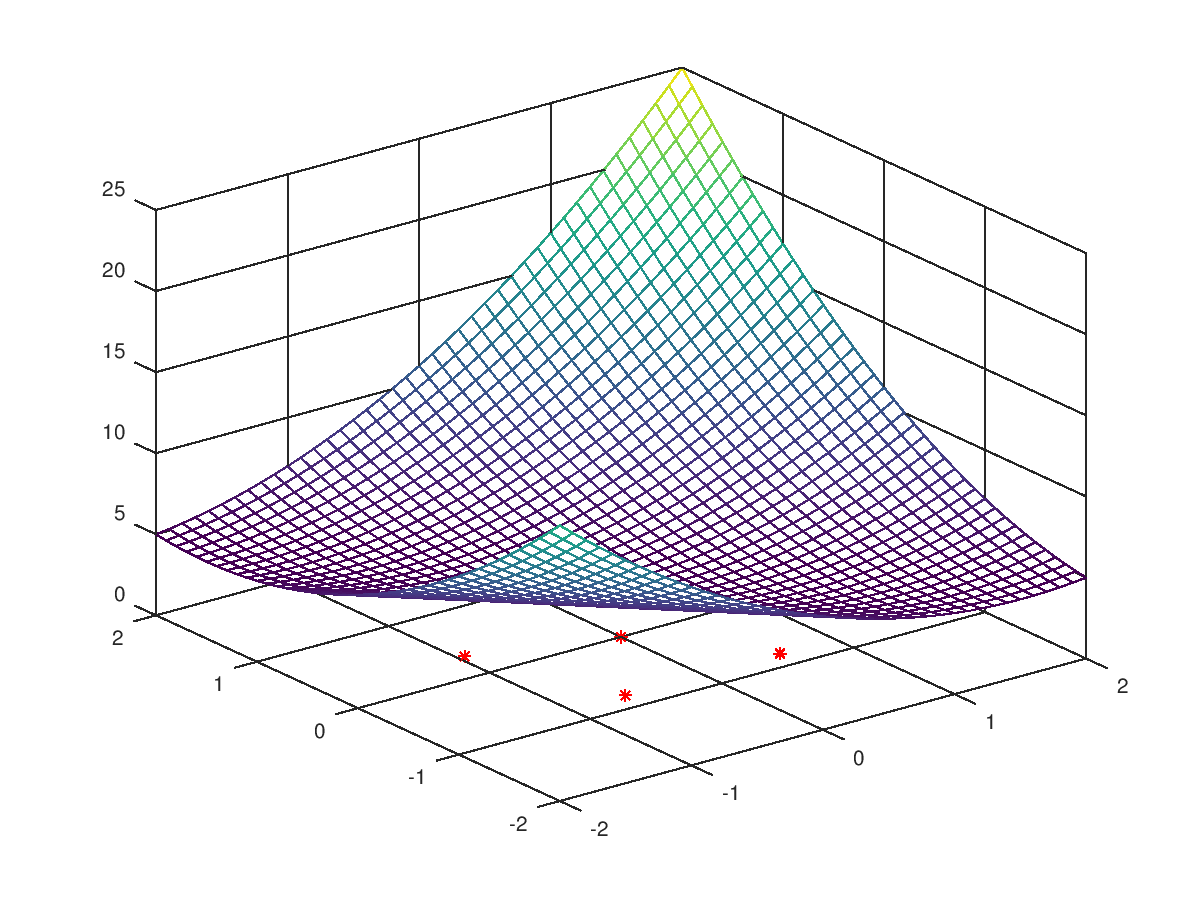
\includegraphics[width=120px]{images/poised_good.png} 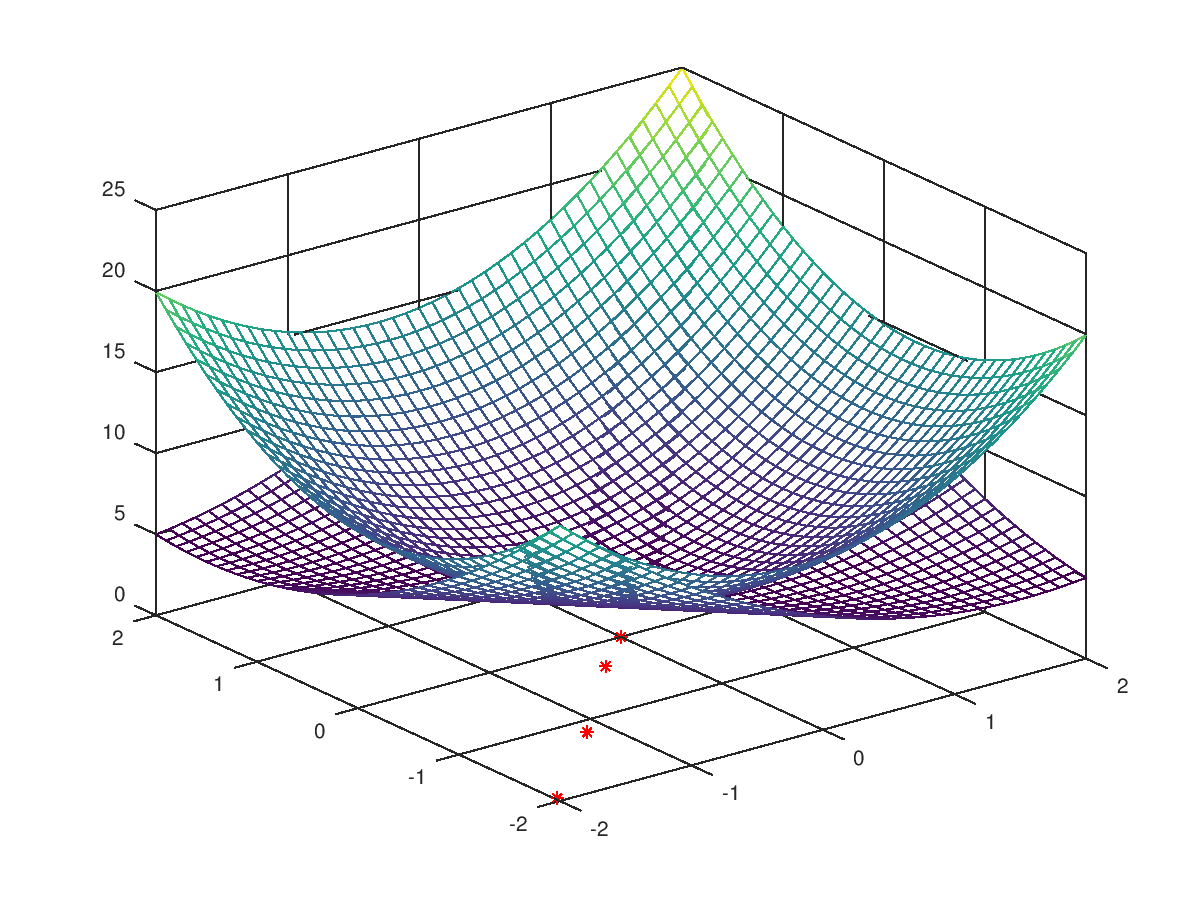
\includegraphics[width=120px]{images/poised_bad.png}
        }
        \item<3> The geometry can be measured by its $\Lambda$-poisedness
        \item<3> Constructing poised sets over ellipses is well known
        \item<3> Constraints limit what points are available for the sample set
        \item<3> With narrow constraints, this means poised sets may not exist
    \end{itemize}
\end{frame}


\section{Convex Always Feasible Algorithm}


\begin{frame}{Feasible Derivative Free Algorithm Part 1}
    \begin{itemize}
        \item We followed an algorithmic template found in \cite{CONEJO2013324}
        \item The template in this article assumes either linear or quadratic models
        \item It describes an algorithm which requires
            \begin{itemize}
                \item An efficiency condition
                \item An accuracy condition
                \item A projection method onto the feasible set
            \end{itemize}
%         \item This algorithm was promising after bench-marking our algorithms on the Hott-Schittowski problem set.
    \end{itemize}
\end{frame}



\begin{frame}{Feasible Derivative Free Algorithm Part 2}
    \begin{itemize}
        \item The efficiency condition requires: $$m_f^{(k)}(x^{(k)}) - m_f^{(k)}(x^{(k+1)}) \ge c_1 \xi^{(k)} \min \{\frac{\xi^{(k)}}{1 + \|\nabla^2 m_f^{(k)}(x^{(k)})\|}, \Delta_k, 1\}$$
        \item This can be satisfied using the Generalized Cauchy Point
        \item The accuracy condition requires: $$\|\nabla m_f^{(k)}(x^{(k)}) - \nabla f (x^{(k)})\| \le c_2 \Delta_k$$
        \item To satisfy this, we require the ellipsoid we find to have bounded condition number
    \end{itemize}
\end{frame}


\begin{frame}{Adoption Difficulties}

\begin{itemize}
    \item We had to modify the convergence analysis to account for projections onto only the linear approximation of the feasible set.
    \item Another difficulty was that the original algorithm does not decrease the trust region radius when accepting the trial point.
    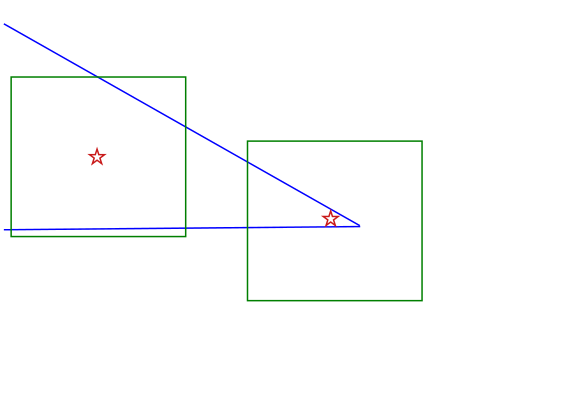
\includegraphics[width=300px]{images/decrease_required.png}
\end{itemize}


\end{frame}


\begin{frame}{Feasible Derivative Free Trust regions}
    \begin{itemize}
        \item We define two trust regions.
        \item The inner trust region:
            \begin{itemize}
                \item Has an ellipsoidal shape
                \item Is assumed to be feasible, with respect to true constraints
                \item Is used for constructing sample points
            \end{itemize}
        \item The outer trust region:
            \begin{itemize}
                \item Is an $L_{\infty}$ ball
                \item Can contain infeasible points, even for the linearization of the constraints
                \item Is used as the search space for computing the next iterate, along with models of the constraints
            \end{itemize}
    \end{itemize}
\end{frame}


\begin{frame}{}
\begin{center}
    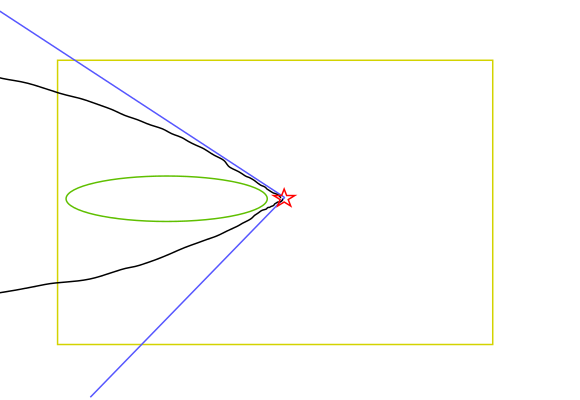
\includegraphics[width=300px]{images/trust_regions.png}
\end{center}
% \includegraphics[width=300px]{images/ellipse_at_current_iterate.png}
\end{frame}



%         \item Use the previous iterations
\begin{frame}{The Algorithm}
    \begin{itemize}
        \item Begin with a feasible set of points
        \item Construct the model functions by evaluating sample points
            \begin{itemize}
                \item Use the previous iteration's models to find a feasible inner trust region
                \item If a point in this ellipsoid is found to be infeasible, decrease the radius
            \end{itemize}
        \item Solve the trust region subproblem
            \begin{itemize}
                \item Add linear constraints to remove infeasible points
            \end{itemize}
        \item Test for sufficient reduction
    \end{itemize}
\end{frame}


\frame {
\frametitle{Extensions to the Algorithm}
\begin{itemize}
    \item The feasible ellipsoid calculation is much more conservative than needed.
    \item We are defining the optimization problem of computing the maximum volume ellipse
    \item There may be simple heuristics that find better ellipsoids
    \item There are different strategies for dealing with infeasible trial points
\end{itemize}

}


\frame {
\frametitle{Adding Linear Cuts to Feasible Region}
\begin{itemize}
    \item There is another strategy for computing the maximal linear shape to be feasible
    \item It could also be convenient for solving the trust region subproblem
    \item The algorithm is as follows:
        \begin{itemize}
            \item Start with a polynomial $p$, a tolerance $\epsilon$, an array of $n_i$ infeasible points $I$, and a set of feasible points $F$.
            \item Compute
            \begin{displaymath}
                \begin{array}{ccccc}
    max_{s, v^{(i)}, b^{(i)}}   & p(s)            &       &                               & \\
                                & p^T v^{(i)}     & \le   & b^{(i)}                       & \forall n \in F, \quad \forall 1 \le i \le m \in n_i\\
                                & I[i]^T v^{(i)}      & \ge   & \epsilon \Delta_k       & \forall 1 \le i \le n_i \\
                                & \|v^{(i)}\|^2   & =     & 1                           & \forall 1 \le i \le n_i \\
                                & I[i]^T v^{(i)}      & \ge   & \epsilon                & \forall 1 \le i \le n_i \\
                                & s          & \in   & B_{\infty}(x^{(k)}, \Delta_k)    & \\
                \end{array}
            \end{displaymath}
        \end{itemize}
\end{itemize}

}


\begin{frame}{}
\begin{center}
    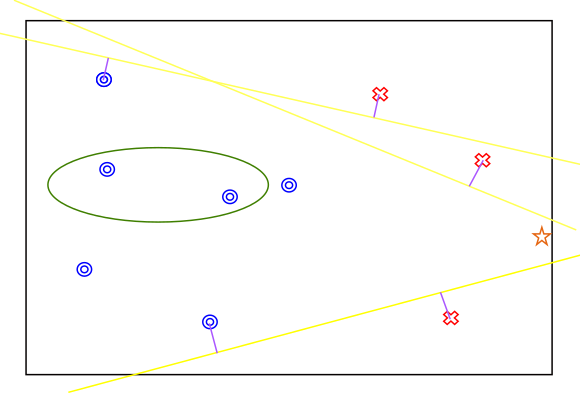
\includegraphics[width=300px]{images/cut_infeasible_points.png}
\end{center}
% \includegraphics[width=300px]{images/ellipse_at_current_iterate.png}
\end{frame}


\frame {
    \frametitle{Questions?}
}

\begin{frame}[allowframebreaks]
    \frametitle{References}
    \bibliographystyle{apalike}
    \bibliography{presentation}
\end{frame}



\section{Future Work}

\frame{
\frametitle{Using Fewer Sample Points}
    \begin{itemize}
        \item With general convex constraints, sufficiently poised sets within the feasible region may not exist.
        \item To illustrate, consider finding a fully quadratic model in 2-dimensions.
        \item As the constraints become more thin,
            \begin{itemize}
                \item The model becomes less poised
                \item There is less need for requiring the model to be quadratic in $y$.
            \end{itemize}
        \item We would prefer to use a subset of all quadratics, with fewer points to approximate them.
    \end{itemize}
}

\frame {
\frametitle{2D Illustration}
    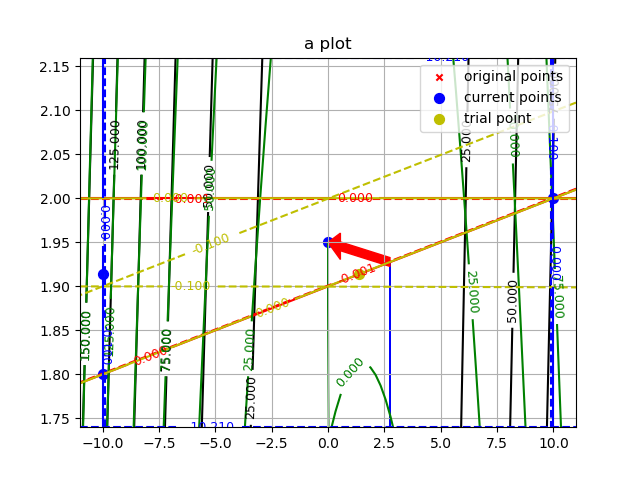
\includegraphics[width=150px]{images/2_2_4_68.png}
    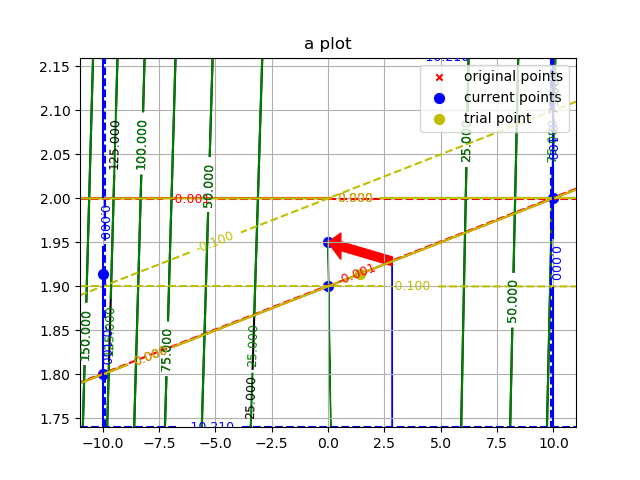
\includegraphics[width=150px]{images/2_3_5_1.png}
}

\frame {
\frametitle{Full pivoting}
    \begin{itemize}
        \item One approach is to use full pivoting within the LU factorization used compute the Lagrange polynomials.

        \item When there are no more pivots greater than a threshold, the LU factorization terminates, and only uses the points and polynomials already computed after zeroing the remaining entries.
        
        \item This method will provide the next point to use as well as the next polynomial to include.
        
    \end{itemize}
}




\end{document}
